\documentclass{article}

% Set page size and margins
% Replace `letterpaper' with`a4paper' for UK/EU standard size
\usepackage[letterpaper,top=2cm,bottom=2cm,left=3cm,right=3cm,marginparwidth=1.75cm]{geometry}

% Useful packages
\usepackage{amsmath}
\usepackage{graphicx}
\usepackage[colorlinks=true, allcolors=blue]{hyperref}

\title{Problem Set 6 - ECON 5253}
\author{Thomas Mondry}

\begin{document}
\maketitle

\section{Data preparation -- J! Archive}

I used this problem set in part to enhance and scale up the data cleaning functions for J! Archive data which I developed in PS5; my primary goal was to create functions that I can use in my final project for acquiring and cleaning the data. Getting the data from the J! Archive HTML pages to the final table which I will use for analysis consists of two steps:

\subsection{Web scraping and data transformation -- complete}

The first part of the process is to convert the data from the HTML elements on the J! Archive site, which are easy to read manually but saved in a terrible format for analysis, into a concise, useful format. This part of the process is nonspecific to any particular research question; I'm just trying to represent all information that is stored in the J! Archive.

This is difficult because the layout of the HTML table containing the clues and the order in which they come up is highly inconsistent, as the tables contain about 40 unnecessary or meaningless cells for each cell containing pertinent information, on average. It is not immediately obvious where to look in the tables in order to find the relevant information; further, in many games, some clues do not get read because time runs out, and the inconsistent formatting of the HTML tables makes it very difficult to identify programmatically whether or not there are missing clues, and if so, which ones these are. However, I have created a set of rules which seem to hold in general. I developed a set of functions (saved in \textbf{/FinalProject/code/scrape.R}) which take a vector of game ID numbers (as have been seemingly arbitrarily selected by the J! Archive admins) and return a single data object, which is a list consisting of three elements:

\begin{enumerate}
	
	\item \textbf{Clue-level information:} A list of length equal to the number of game IDs in the vector; each element is a data frame with 60 rows corresponding to the 30 Jeopardy round and 30 Double Jeopardy round clues, and each row contains information about the round, category, dollar value, and content of the clue; the order in which that clue came up in the game; whether or not that clue is a Daily Double and, if so, the amount of the wager; and each player's performance on that clue (correct, incorrect or no answer)
	
	\item \textbf{Player-level information:} A list of length equal to the number of game IDs in the vector; each element is a data frame with 3 rows corresponding to the 3 players in the game, and each row contains information about the player's name, occupation, scores after the Jeopardy and Double Jeopardy rounds, Final Jeopardy wager, performance on Final Jeopardy (correct or incorrect), final score, and Coryat score (a metric which neither rewards nor punishes aggressive or conservative betting behavior, and which disregards Final Jeopardy)
	
	\item \textbf{Game-level information:} A data frame of row length equal to the number of game IDs in the vector; each row contains some basic information about the game as well as the Final Jeopardy category and clue, which do not have a natural place elsewhere but may be useful
	
\end{enumerate}

For this problem set, I ran the data scraping process on 100 consecutive "regular" (i.e., not from a special tournament) games of \textit{Jeopardy!} from the 2001-2002 season in order to generate some data for visualization. The data object is stored in \textbf{jData\_100games.rda}, which is saved both in the directory for this problem set and in /FinalProject/data.

\subsection{Problem-specific data cleaning -- in progress}

Once I select a research question, I will use my data object (with a larger sample of games for the final project) to create a tabular dataset of revelant features which I can then use to attempt to model the outcome. Since I don't yet have a problem in mind, I didn't create a full data cleaning process for this problem set; however, as shown in the \textbf{PS6\_Mondry.R} script and described below, I did calculate a few metrics for visualizations. For these visualizations, I omitted the 15 of the 100 games in the sample which had more than 4 missing clues (out of 60).

\section{Three visualizations}

\subsection{Relationship between Coryat score and true post-Double Jeopardy score}

A player's Coryat score (a concept developed by former \textit{Jeopardy!} champion Karl Coryat) is defined as the score they would have after the first two rounds of the game if Daily Double wagers were fixed to the underlying point value of the clue. So, for example, if a player found a Daily Double in a \$1,600 clue in the Double Jeopardy round, wagered \$3,000, and answered correctly, their true score would increase by \$3,000; however, their Coryat score would only increase by \$1,600; Coryat scores work the same way if a player answers a Daily Double incorrectly. The Coryat score was intended for viewers to follow along at home and measure their performance in games, but is also a useful metric for separating betting strategy from game scores. A large difference between Coryat score and true post-Double Jeopardy score is generally an indicator of aggressive betting.

\smallskip

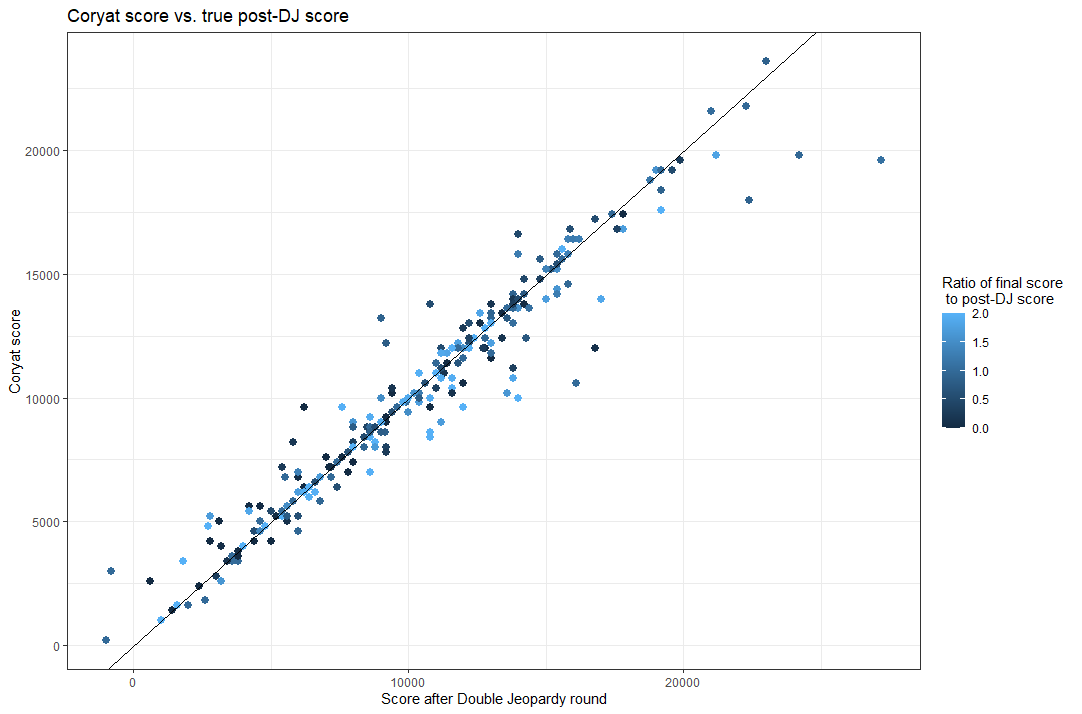
\includegraphics[width=\textwidth]{PS6a_Mondry.png}

\smallskip

This plot shows the extent of this difference as observed in all 3 players from all 85 games in the data, relative to a perfectly neutral wagering strategy (on average) which is represented by the line with unit slope. Points to the right of the line correspond to successful aggressive wagering, while points to the left of the line correspond to unsuccessful aggressive wagering.

Final Jeopardy wagers cannot be considered generally indicative of either skill nor risk preferences, since in practice players tend to select their wagers deterministically based on their standing relative to their opponents. However, I wanted to see if there appears to be any correlation between the success of earlier aggressive wagers and the success of large Final Jeopardy wagers using the color scale. We can observe that many points to the right of the line correspond to large gains in the final round, and many points to the left correspond to large losses; however, this effect does not appear to be very pronounced, and there are many exceptions.

\subsection{Final Jeopardy wagers by post-Double Jeopardy ranking}

To get a better idea of how Final Jeopardy wagering behavior could be modeled, I looked at the sample distributions of Final Jeopardy wagers for players in each ranking going into the Final Jeopardy round. This information is represented in this plot:

\smallskip

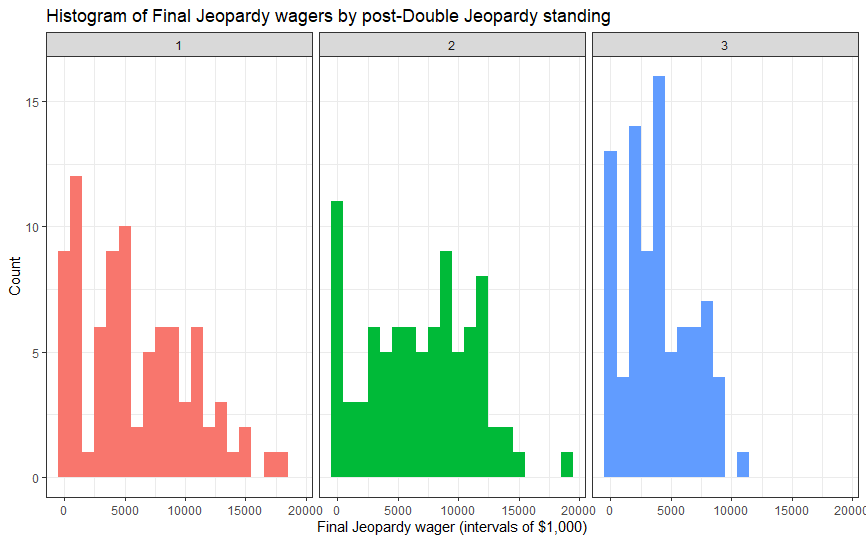
\includegraphics[width=\textwidth]{PS6b_Mondry.png}

\smallskip

This is a smaller sample than I would ideally want to use, as the histograms are pretty choppy, but we can observe some general differences. Players which lead the game going into the final round are more likely to make smaller wagers, in comparison to players that are in second place. Interestingly, players in last place going into Final Jeopardy also make small wagers in a high proportion of cases, but because this metric is an absolute dollar amount, this could be because last-place players have less money to wager.

\subsection{Relationship between large Final Jeopardy wagers and final placement}

Of the 255 players in the data, 84 wagered more than 90\% of their pre-Final Jeopardy money in Final Jeopardy. I wanted to see how the final placement outcomes differ for these players, compared to those who wagered more conservatively.

\smallskip

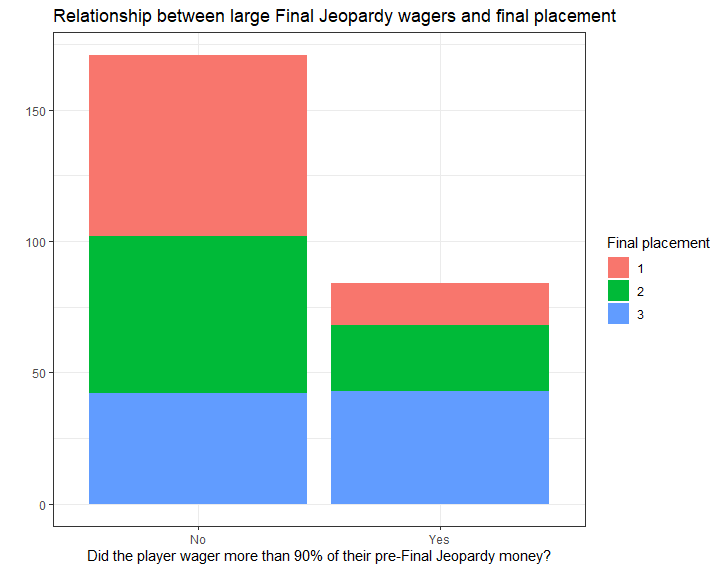
\includegraphics[width=5in]{PS6c_Mondry.png}

\smallskip

As expected, players who make large wagers are proportionally much less likely to win than those who don't. This is likely due in large part to the fact that the necessity of making a large wager often indicates that a player is either well behind the other players, in which case they are unlikely to score enough points to win, or that the player has a narrow lead, which makes Final Jeopardy more of a 50/50 gamble. Interestingly, the proportional likelihood of placing second is about the same whether or not the wager was very large. This may be because in games where large wagers are necessary for any player, they are frequently necessary for more than one player, so one of the players who makes a large wager is likely to place second.

\end{document}